% This must be in the first 5 lines to tell arXiv to use pdfLaTeX, which is strongly recommended.
\pdfoutput=1
% In particular, the hyperref package requires pdfLaTeX in order to break URLs across lines.

\documentclass[11pt]{article}

% Remove the "review" option to generate the final version.
\usepackage[review]{acl}

% Standard package includes
\usepackage{times}
\usepackage{latexsym}

% For proper rendering and hyphenation of words containing Latin characters (including in bib files)
\usepackage[T1]{fontenc}
% For Vietnamese characters
% \usepackage[T5]{fontenc}
% See https://www.latex-project.org/help/documentation/encguide.pdf for other character sets

% This assumes your files are encoded as UTF8
\usepackage[utf8]{inputenc}

% This is not strictly necessary, and may be commented out,
% but it will improve the layout of the manuscript,
% and will typically save some space.
\usepackage{microtype}

\usepackage{times}
\usepackage{latexsym}

% For proper rendering and hyphenation of words containing Latin characters (including in bib files)
\usepackage[T1]{fontenc}
% For Vietnamese characters
% \usepackage[T5]{fontenc}
% See https://www.latex-project.org/help/documentation/encguide.pdf for other character sets

% This assumes your files are encoded as UTF8
\usepackage[utf8]{inputenc}
\usepackage{booktabs}

\usepackage{epsfig}
\usepackage{graphicx}
\usepackage{amsmath}
\usepackage{amssymb}
\usepackage{enumitem}
\usepackage{tabularx}
\usepackage{multirow}
\usepackage{epsfig}

\graphicspath{ {./images/} }
\usepackage[rightcaption]{sidecap}
\usepackage[export]{adjustbox}
\usepackage{wrapfig}

% This is not strictly necessary, and may be commented out,
% but it will improve the layout of the manuscript,
% and will typically save some space.
\usepackage{microtype}

\usepackage{hyperref}

% If the title and author information does not fit in the area allocated, uncomment the following
%
%\setlength\titlebox{<dim>}
%
% and set <dim> to something 5cm or larger.

\title{Language Guided Navigation in Dynamic Environment}

% Author information can be set in various styles:
% For several authors from the same institution:
% \author{Author 1 \and ... \and Author n \\
%         Address line \\ ... \\ Address line}
% if the names do not fit well on one line use
%         Author 1 \\ {\bf Author 2} \\ ... \\ {\bf Author n} \\
% For authors from different institutions:
% \author{Author 1 \\ Address line \\  ... \\ Address line
%         \And  ... \And
%         Author n \\ Address line \\ ... \\ Address line}
% To start a seperate ``row'' of authors use \AND, as in
% \author{Author 1 \\ Address line \\  ... \\ Address line
%         \AND
%         Author 2 \\ Address line \\ ... \\ Address line \And
%         Author 3 \\ Address line \\ ... \\ Address line}

\author{First Author \\
  Affiliation / Address line 1 \\
  Affiliation / Address line 2 \\
  Affiliation / Address line 3 \\
  \texttt{email@domain} \\\And
  Second Author \\
  Affiliation / Address line 1 \\
  Affiliation / Address line 2 \\
  Affiliation / Address line 3 \\
  \texttt{email@domain} \\}

\begin{document}
\maketitle
\begin{abstract}
 Navigation in the dynamically changing real world is a challenging task, and conditioning it on linguistic commands makes it an even more challenging problem. Humans effortlessly perform language-guided navigation in their daily lives, and with this work, we take a step towards imparting autonomous vehicles with similar capabilities. In order to perform language-guided navigation in the dynamic world, we need to simultaneously reason about the linguistic command and the dynamic visual world, both temporally and spatially. To this end, we propose a novel language grounding model that localizes the goal region corresponding to the language command and provides interpretable intermediate trajectory predictions to navigate towards the goal region. Additionally, we release a novel video-language navigation meta-dataset in the Carla environment. We provide extensive quantitative and qualitative empirical results to validate the effectiveness of our approach. Finally, we perform real-time efficacy of the proposed approach.
\end{abstract}

%%
%% The code below is generated by the tool at http://dl.acm.org/ccs.cfm.
%% Please copy and paste the code instead of the example below.
%%
% \begin{CCSXML}
% <ccs2012>
%  <concept>
%   <concept_id>10010520.10010553.10010562</concept_id>
%   <concept_desc>Computer systems organization~Embedded systems</concept_desc>
%   <concept_significance>500</concept_significance>
%  </concept>
%  <concept>
%   <concept_id>10010520.10010575.10010755</concept_id>
%   <concept_desc>Computer systems organization~Redundancy</concept_desc>
%   <concept_significance>300</concept_significance>
%  </concept>
%  <concept>
%   <concept_id>10010520.10010553.10010554</concept_id>
%   <concept_desc>Computer systems organization~Robotics</concept_desc>
%   <concept_significance>100</concept_significance>
%  </concept>
%  <concept>
%   <concept_id>10003033.10003083.10003095</concept_id>
%   <concept_desc>Networks~Network reliability</concept_desc>
%   <concept_significance>100</concept_significance>
%  </concept>
% </ccs2012>
% \end{CCSXML}

% \ccsdesc[500]{Computer systems organization~Embedded systems}
% \ccsdesc[300]{Computer systems organization~Redundancy}
% \ccsdesc{Computer systems organization~Robotics}
% \ccsdesc[100]{Networks~Network reliability}

%%
%% Keywords. The author(s) should pick words that accurately describe
%% the work being presented. Separate the keywords with commas.
% \keywords{datasets, neural networks, gaze detection, text tagging}

%% A "teaser" image appears between the author and affiliation
%% information and the body of the document, and typically spans the
%% page.
% \begin{teaserfigure}
%   \includegraphics[width=\textwidth]{sampleteaser}
%   \caption{Seattle Mariners at Spring Training, 2010.}
%   \Description{Enjoying the baseball game from the third-base
%   seats. Ichiro Suzuki preparing to bat.}
%   \label{fig:teaser}
% \end{teaserfigure}

%%
%% This command processes the author and affiliation and title
%% information and builds the first part of the formatted document.
\maketitle

\section{Introduction}

\begin{figure}[!t]
    \centering
    \begin{tabular}[t]{p{0.48\textwidth} }
    { \centering \small {\textit{\textbf{Command: }``Stop for the traffic light and then take a right and park near the bus stand.''}}}\\
        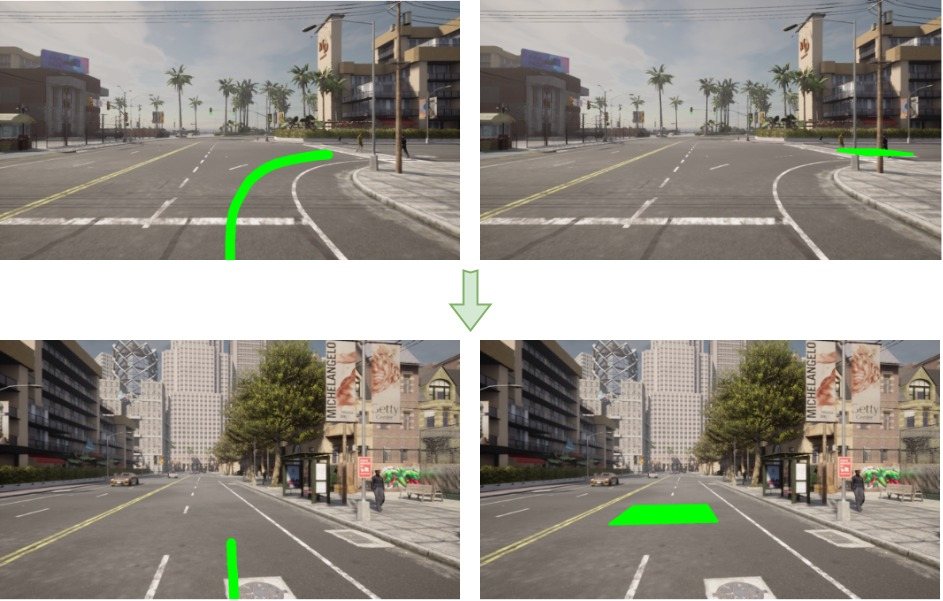
\includegraphics[width=0.48\textwidth]{images/teaser.jpg} \\
    \end{tabular}
    \caption{A dataset sample from the proposed CARLA-Nav dataset. For the given command, the ground truth of the dataset consists of navigable regions corresponding to "taking a right" and "park near the bus stand" and the corresponding trajectories to reach the navigable regions. }
    \label{fig:teaser}
\end{figure}

Humans have exceptional navigational abilities, which, combined with their visual and linguistic prowess, allow them to perform navigation based on the linguistic description of the objects of interest in the environment. This is in direct consequence of the human capability to associate visual objects with their linguistic descriptions. Referring Expression Comprehension (REC) and Referring Image Segmentation (RIS) are two tasks for associating the visual objects based on their linguistic descriptions using bounding-box-based and pixel-based localizations, respectively. However, it is non-trivial to utilize these localizations directly for a navigation task. For example, consider the linguistic command "take a right turn from the intersection," an object-based localization is not usable for navigation as it doesn't answer the question "which region" on the road to navigate to. To solve the aforementioned issue, the task of Referring Navigable Regions (RNR) was proposed in \cite{Rufus_2021} to localize the navigable regions in a static front camera image on the road corresponding to the linguistic command. However, grounding the linguistic expression in a single image is problematic, as it is possible that the object referred to in the natural language expression is not visible, is occluded, or goes out of frame as the vehicle moves. Consider the example in Figure \ref{fig:teaser}, and the "right turn" is not visible in the image; as a result, the RNR-based approach gives a meaningless output that is not correlated with the linguistic command. Furthermore, in a dynamically changing environment, these kinds of issues are highly prevalent, and the vanilla RNR approach designed for static images fails. In this work, we re-formulate the RNR approach to perform language-guided navigation in a dynamically changing environment by grounding intermediate navigable regions when the referred navigable region is not visible.

Over the past years, there have been numerous approaches for language-guided navigation in both indoor and outdoor environments. Existing works \cite{anderson2018vision, https://doi.org/10.48550/arxiv.2001.02330, https://doi.org/10.48550/arxiv.1810.00663} on indoor navigation assume that the navigational environment is fully known. This allows them to discretize the known map into a graphical representation, where the nodes are the set of navigable regions (landmarks) that the agent can navigate given the linguistic command. However, this approach is not practical for outdoor settings where the environment is not known. Touchdown \cite{chen2019touchdown} is a popular benchmark dataset for outdoor language-based navigation. It consists of pre-recorded google street view images and allows navigation across street views by choosing from a set of discrete actions \cite{schumann-riezler-2022-analyzing, zhu-etal-2021-multimodal, xiang-etal-2020-learning}. Current approaches for indoor and outdoor settings model the task of vision language navigation as a sequence-to-sequence prediction \cite{sriram2019talk, schumann-riezler-2022-analyzing, zhu-etal-2021-multimodal} or as a reinforcement learning problem \cite{anderson2018vision, fu2019language}. For a given linguistic command, they predict a sequence of actions or behaviors to perform navigation in the environment. However, discretizing the action space and the environment limits the type of navigational maneuvers that can be performed. For example, consider the command, "park between the two cars on the right", a discrete action space doesn't provide fine-grained control of the car, and a discrete environment limits the kind of navigable regions to execute the given command successfully. The aforementioned issues become apparent in a dynamically changing environment, where fine-grained control of the car's navigation and a fully navigable environment is required to adapt to the dynamic surroundings and perform navigational maneuvers based on the linguistic command. In this paper, we present a novel meta-dataset in the CARLA environment for outdoor navigation which addresses the limitations associated with the existing navigation datasets. Additionally, the visual grounding-based approach allows us to have a fine-grained control over the vehicle as it enables navigation to any drivable region on the road.

Another limitation of the current sequence-to-sequence and reinforcement learning approaches is that their predictions are not interpretable. It is non-trivial to understand their predictions as there is no feedback. Instead, in the visual-grounding-based approach, there is visual feedback associated with each prediction in terms of the segmentation mask corresponding to the navigable region on the road. Furthermore, we also predict the intermediate trajectories depicting the vehicle's navigation path. Consequently, we propose a novel multi-task network that predicts interpretable segmentation masks for intermediate trajectory and navigable region prediction tasks. Moreover, we perform real-time inference on the proposed meta-dataset. To the best of our knowledge, this is the first attempt towards language-based navigation in outdoor environments in real-time. Lastly, we conduct comprehensive qualitative and quantitative ablations to validate the effectiveness of our approach.

%% Introduce the problem / describe the problem statement
% Humans have exceptional navigational abilities, which, combined with their visual and linguistic prowess, allow them to perform navigation based on the linguistic description of the objects of interest in the environment. This is in direct consequence with the human capability of associating visual objects with their linguistic descriptions. Referring Expression Comprehension and Referring Image Segmentation are two tasks for associating the visual objects based on their linguistic descriptions using bounding-box based and pixel-based  





% Humans have exceptional navigational abilities, which, combined with their visual and linguistic prowess, allow them to perform navigation based on the linguistic description of the objects of interest in the environment. This is in direct consequence with the human capability of associating visual objects with their linguistic descriptions. The task of visual grounding is concerned with localizing objects or regions in an image based on a natural language query. Visual grounding is a critical part of language-guided navigation as the first step involves comprehending the linguistic instruction and then performing localization based on it. In autonomous navigation, this problem is formally known as Referring Navigable Regions (RNR)~\cite{Rufus_2021}, and the goal is to ground navigable regions in an image based on the linguistic command. However, in practice it is not feasible to work with static images as it is possible that the object referred to in the natural language expression is not visible, is occluded or goes out of frame as the vehicle moves. Consider a simple command ``Take the next right", now the right turn may not be immediately visible and the model should have ability to make intermediate predictions. 

% In this work, we re-formulate the RNR task to perform language-guided navigation in a dynamically changing environment instead of static images.

% Humans have exceptional navigational abilities, which, combined with their visual and linguistic prowess, allow them to perform navigation based on the linguistic description of the objects of interest in the environment. This is in direct consequence with the human capability of associating visual objects with their linguistic descriptions. The task of visual grounding is concerned with localizing objects or regions in an image based on a natural language query. Visual grounding is a critical part of language-guided navigation as the first step involves comprehending the linguistic instruction and then performing localization based on it. In autonomous navigation, this problem is formally known as Referring Navigable Regions (RNR)~\cite{Rufus_2021}, and the goal is to ground navigable regions in an image based on the linguistic command. In this work, we extend the task of RNR to perform language grounding over a dynamically changing scene; additionally, we predict interpretable intermediate trajectories to reach the final destination region referred by the linguistic command.


% discreete output space
% map / graph is known, not applicable in dynamic environment
% pre-recorded sequences
% discrete 


% why is visual grounding approach better than others and their limitations
% make distinction b/w outdoor and indoor
% Existing approaches to language-guided navigation model the task as a sequence-to-sequence prediction problem \cite{schumann-riezler-2022-analyzing, chen2019touchdown, zhu-etal-2021-multimodal, xiang-etal-2020-learning} or as a reinforcement learning problem \cite{fu2019language, nguyen2019vision, anderson2018vision}. They predict a sequence of behaviors or actions from the given linguistic command and visual cues from the environment. The linguistic commands used by these approaches are lengthy, complicated, and unrealistic; however, it is non-trivial to interpret the network prediction for such commands. Additionally, these approaches fail miserably \cite{schumann-riezler-2022-analyzing} when a short and straightforward command is passed as input. In this paper, we take a visual-grounding-based approach to language-guided navigation, which has been previously explored in \cite{deruyttere2019talk2car, rufus2020cosine, Rufus_2021}. \cite{deruyttere2019talk2car, rufus2020cosine} predict a bounding-box corresponding to the object referred to in the linguistic command. However, localizing the referred object in an image is not directly amenable for navigational purposes as the ambiguity regarding ``which region on the road" to navigate persists. Instead, \cite{Rufus_2021} ground the navigable regions on the road corresponding to the command, which an external motion planner can directly utilize for navigation.

% The problem with existing visual-grounding-based approaches is that they utilize a single image and the linguistic command as input to their network. Single image input is not suitable for the task, as it is impossible to ground regions/objects that are not in view. For example, the command in Figure \ref{fig:teaser} requires identifying the navigable regions on the road for ``take a right" and a region near the bus stand for ``park near the bus stand." However, the bus stand is not visible at the time the language command is given and will only be visible once a right turn has been taken. Therefore, instead of grounding navigable regions on a single image, we propose to ground navigable regions over a video input. For the command in Figure \ref{fig:teaser}, we separately ground navigable regions corresponding to "stop for the traffic light," "take a right turn," and "park near the bus stand."

% what are we doing? / our contributions. 
% this point is invalid as many approaches perform navigation in simulator environment.
% we reformulate the RNR task for dynamic environments
% we propose a novel multi task network, our approach in interpretable.
% we propose a novel outdoor meta-dataset/tool on CARLA simulator.
% we perform real-time evaluation on outdoor navigation.
% showcase comprehensive qualitative and quantitative experimental results.



% Another limitation of existing approaches is that they perform the evaluation on pre-recorded sequences from the dataset. 



% this is not good as it doesn't capture the situation in real-world where 

% where we predict segmentation masks corresponding to navigable regions on road and intermediate trajectories for the linguistic command, which can be easily interpreted to understand the network prediction.

% Why are we solving the problem? compare with previous RNR work
% It is commonplace for humans to utilize fine-grained linguistic instructions for executing navigational maneuvers in real-time. Consider the scenario of a passenger in a taxi; the passenger instructs, "turn right from the intersection and stop near the bus stand." 



% The taxi driver must make simultaneous temporal and spatial decisions by asking `When?' and  `Where?'. He has to make real-time decisions regarding `when' to turn right and stop, and `where' to stop. From the RNR perspective, it requires identifying the navigable regions on the road for ``turning right" and a region near the bus stand for ``stopping". However, \cite{Rufus_2021} 

% The linguistic commands used by these approaches are long and complicated, ex: ``Head straight until you come to a traffic light with Starbucks to your far left corner. Turn left. At the next light with Capital One on your far right corner, turn right and stop."

% however the sequence is only the text and in the visual modality only static images are taken as input. 

% It is commonplace for humans to utilize fine-grained linguistic instructions for executing navigational maneuvers in real-time. Consider the scenario of a passenger in a taxi; the passenger instructs, "turn right from the intersection and stop near the bus stand." The taxi driver must make simultaneous temporal and spatial decisions by asking `When?' and  `Where?'. He has to make real-time decisions regarding `when' to turn right and stop, and `where' to stop. From the RNR perspective, it requires identifying the navigable regions on the road for ``turning right" and a region near the bus stand for ``stopping."



% Existing approaches on language-guided navigation can be divided into two categories: (1) Sequential Approach, and (2) Visual Grounding-based approach.

% Link with visual grounding then add limitations of other datasets
% It is commonplace for humans to utilize fine-grained linguistic instructions for executing navigational maneuvers in real-time. Consider the scenario of a passenger in a taxi; the passenger instructs, "turn right from the intersection and stop near the bus stand." The taxi driver must make simultaneous temporal and spatial decisions by asking `When?' and  `Where?'. He has to make real-time decisions regarding `when' to turn right and stop, and `where' to stop. From the RNR perspective, it requires identifying the navigable regions on the road for ``turning right" and a region near the bus stand for ``stopping." 

% Motivation behind the problem
% It is commonplace for humans to utilize fine-grained linguistic instructions for executing navigational maneuvers in real-time. Consider the scenario of a passenger in a taxi; the passenger instructs, "turn right from the intersection and stop near the bus stand." The taxi driver must make simultaneous temporal and spatial decisions by asking `When?' and  `Where?'. He has to make real-time decisions regarding `when' to turn right and stop, and `where' to stop. From the RNR perspective, it requires identifying the navigable regions on the road for ``turning right" and a region near the bus stand for ``stopping." Now, suppose the distance between the `bus stand' and the current location is considerable; this scenario becomes particularly challenging as it requires the taxi to keep moving until a `bus stand" becomes visible and then `stop" at a region near it. Our novel dataset consists of multiple such scenarios, which require strong temporal reasoning to successfully navigate to the desired location.

% While several reinforcement learning-based approaches for language-based navigation exist, they incorporate discrete actions in their Markov decision process formulation. This setting is limited and impractical in realistic scenarios where actions form a continuous space rather than a discrete one. We adopt a visual grounding-based approach to explicitly specify the navigable regions on the road corresponding to the linguistic command.\cite{Rufus_2021} take a similar approach, but their work only considers image-language pairs for the navigational purpose, and they do not explicitly show live navigation towards the goal region. Instead, we utilize dynamic scenes through video-language pairs to continuously ground the navigable region on the road corresponding to the language command. Additionally, the intermediate trajectory predictions guide the navigation towards the goal region. The entire approach is end-end trainable and promises a new paradigm shift in language-based navigation literature, which is more focused on the visual grounding aspect.

% Our Approach & Contributions
% To this end, we propose a novel multi-task network for navigable region prediction and trajectory prediction in a dynamic scene. We explicitly distinguish between intermediate regions and final goal regions for navigable region prediction. The predicted trajectory is interpretable and used to navigate towards the predicted final goal region. Additionally, we propose a novel video-language Navigation meta-dataset in the Carla environment. The proposed dataset is the first of its kind, and it consists of video-language pairs with frame-level annotations. We benchmark the dataset with our novel multi-task network and provide extensive quantitative and qualitative ablation to validate our approach. Finally, we showcase the viability of the proposed approach by performing real-time inference in the Carla environment and successfully executing the language command by navigating to the final goal region based on the trajectory predictions.

% We propose a novel approach to natural language-guided navigation in dynamic outdoor environments. We present an outdoor language-guided navigation tool on the CARLA simulator with direct control over the various environmental parameters. Per-frame navigable regions with future trajectory predictions are provided for a linguistic command. A novel multi-task network that predicts interpretable segmentation masks for intermediate trajectory and navigable region prediction tasks is presented. To the best of our knowledge, we are the first ones to perform a real-time inference on outdoor environments for the task vision language navigation. Finally, we conduct comprehensive qualitative and quantitative ablations to validate the effectiveness of our approach.

To summarize, the main contributions of this paper are the following:
\begin{itemize}
\item We present a vision language navigation tool on CARLA simulator which provides fine-tuned control of the vehicle to execute various language-base navigational manoeuvres.
\item We propose a novel multi-task network for trajectory prediction and per-frame RNR tasks in dynamic outdoor environments. The prediction for each task is explainable and interpretable in the form of segmentation masks.
\item We perform real-time navigation in the CARLA environment with a diverse set of linguistic commands.
\item Finally, extensive qualitative and quantitative ablations are performed to validate the practicality of our approach.  


% \item We propose a novel multi-task network for predicting navigable regions and intermediate trajectories in a dynamic scene. The prediction for each task is explainable and interpretable in the form of segmentation masks.
% \item We present a novel meta-dataset, CARLA-NAV, for video-language navigation task. The dataset is curated using the open source Carla Simulator.
% \item We benchmark the dataset using our novel multi-task network and perform extensive ablation studies.
% \item We perform real-time language-based navigation with the proposed multi-task network in the Carla environment. We utilize the network predictions and a local planner to successfully navigate the final goal region.

\end{itemize}


\section{Related Work}

\subsection{Visual Grounding}

Visual grounding aims to help associate the linguistic description of entities with their visual counterparts by localizing them visually. There are two prevalent approaches for visual grounding based on the type of localization used. Proposal-based localization is formally referred to as Referring Expression Comprehension (REC). Most methods in REC follow a propose-then-rank strategy, where the ranking is done using similarity scores \cite{rohrbach2016grounding, hu2016natural, plummer2018conditional, rufus2020cosine} or through attention-based methods \cite{deng2018visual, zhang2018grounding, yang2019dynamic, qiu2020language}. The other approach is to localize the objects by their pixel-level segmentation mask, formally known as Referring Image Segmentation (RIS). In RIS, methods use different strategies to fuse the spatial information of the image with the word-level information of the language query \cite{shi2018key, ye2019cross, huang2020referring, jain2021comprehensive}. However, in the context of autonomous navigation, both REC and RIS are limited because they localize the objects, but the problem of how to navigate towards the object still persists. Recently, \cite{Rufus_2021} proposed the Referring Navigable Region (RNR) task to localize the navigable regions on the road corresponding to the language commands. However, they showcase results on a static image, and they don't show the actual navigation in a dynamic environment. Instead, we propose to reformulate the RNR task for dynamic outdoor settings and perform real-time navigation based on language commands.

\subsection{Language-based Navigation}

The objective of language-guided navigation is to allow humans to have the capability to control and influence the navigation of autonomous agents through language commands. Existing Works have utilized imitation learning \cite{nguyen2019vision, nguyen2019help}, behavior cloning \cite{das2018neural}, sequence-sequence translation \cite{anderson2018vision}, and cross-modal attention \cite{huang2019multi, irshad2021hierarchical, cornia2019perceive} based approaches. Most of the literature has focused on indoor environments; both synthetic \cite{kempka2016vizdoom, kolve2017ai2, wu2018building}, and real \cite{chang2017matterport3d, anderson2018vision}. While there are many papers \cite{mirowski2018learning, chen2019touchdown, chancan2020citylearn} on autonomous navigation in outdoor environments, very few of them \cite{sriram2019talk} perform language-based navigation in an outdoor setting. Specifically, \cite{sriram2019talk} predict local waypoints conditioned on the language command to generate trajectories for navigation, but the language commands used by them have less diversity. In this paper, we use diverse linguistic commands with detailed visual descriptions. Additionally, we propose a paradigm shift towards utilizing RNR-based approaches for language-guided navigation, and the CARLA-NAV meta-dataset proposed in this paper is a step towards achieving this goal. 

\section{Dataset}

% This is a meta-dataset, we release the toolkit which can be further used to extend dataset.
% This dataset is first of it's kind and proposes a paradigm shift

The proposed CARLA-NAV dataset was curated using the open-source Carla Simulator for autonomous driving research. It contains episodic level data, where each episode consists of language commands and the corresponding video from Carla Simulator of navigation towards the final goal region described by the command. Each frame from the video is annotated with a segmentation mask corresponding to the intermediate and final navigable regions. The intermediate masks capture the navigable regions traversed by the vehicle until reaching the final goal region corresponding to the language command. Furthermore, we also record the 3D vehicle position in the Carla environment and the camera intrinsic-extrinsic matrices for each frame. For the trajectory prediction task, we take the 3D vehicle position of the vehicle in the successive frames and project the 3d positions to the front-camera image using the projective transformation. We treat trajectory prediction as a dense prediction task to make it interpretable during navigation. 

The dataset includes video sequences captured in 8 different maps, 14 distinct weather conditions, and a diverse range of vehicles and passengers in the environment. The language commands in our dataset contain detailed visual descriptions of the environment and describe a wide range of maneuvers. In some cases, there are multiple maneuvers in a single command. Overall, the training split of the dataset consists of 500 video-language pair sequences, and the validation split consists of 50 sequences. In the next section, we describe the dataset creation process.

\begin{figure*}[t]
\centering
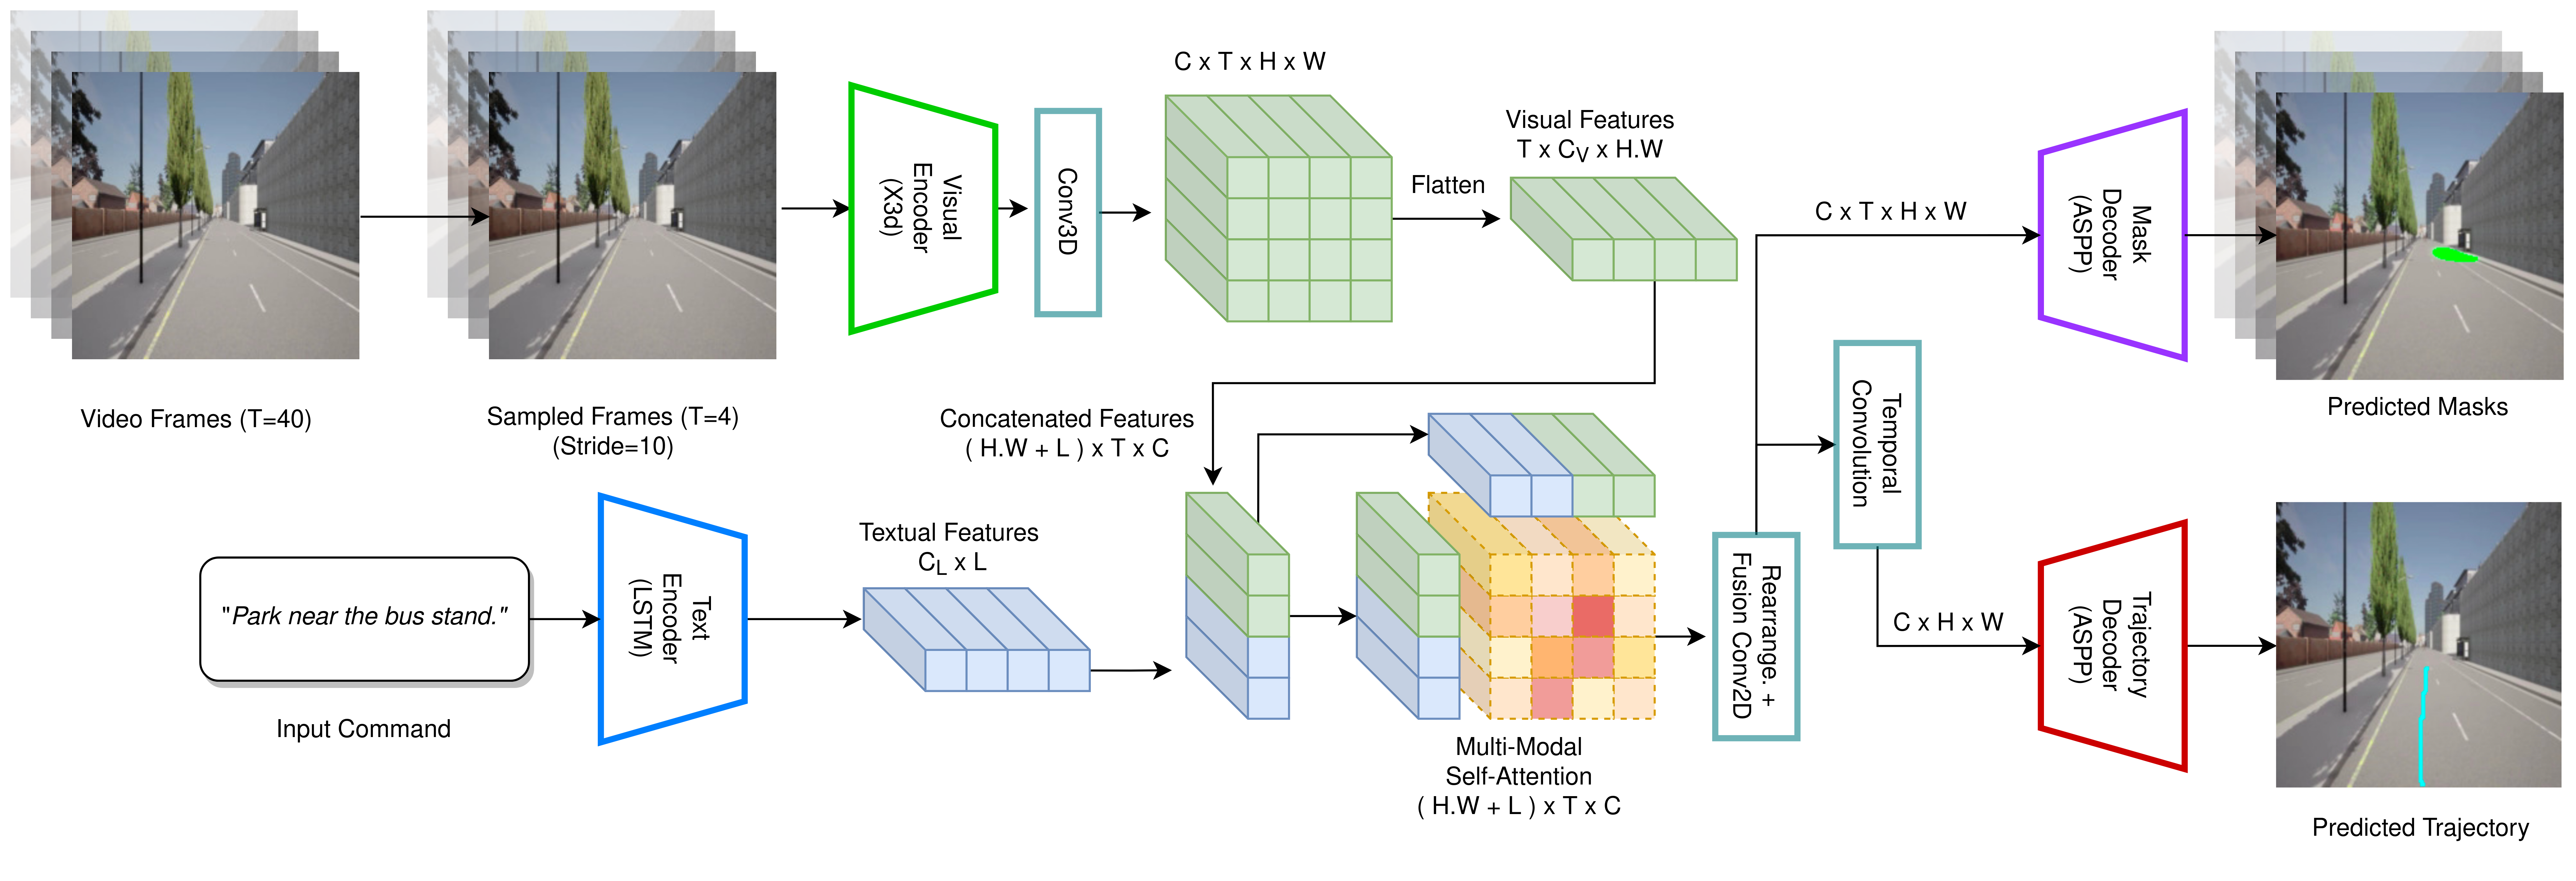
\includegraphics[width=1.0\textwidth]{images/Conv3D_Model.png}
\caption{TODO: Add suitable caption to network architecture.}
\label{proposed_pipeline}
\end{figure*}

\subsection{Dataset Creation}

% todo: 25 validation + 25 test

% defend rule-based planner? command before or after
We created a data-collection toolkit on top of Carla's API and plan to open-source it upon acceptance. The data collection process can be grouped into two steps: (1) providing a language command that describes the series of navigational maneuvers and (2) navigating the Carla environment based on the language command. Next, we describe each step in detail.
The language commands for navigation were provided manually through a text prompt and were in direct correspondence with the surrounding environment. For navigation, we used mouse clicks to select the navigable regions for the vehicle in the front camera view of the RGB camera and get the 2D point corresponding to the click. We use a depth camera to get the depth corresponding to the 2D pixel and then transform it to the 3D world coordinates using Inverse Projective transform; this 3D position is passed as input to the local planner to navigate the Carla environment. We use a simple rule-based planner for our case; however, this can easily be replaced with more advanced planners like RRT and RRT*. For the trajectory prediction task, we take the 3D vehicle position of the vehicle in the successive frames and project the 3D positions to the front-camera image using the projective transformation. We treat trajectory prediction as a dense prediction task to make it interpretable during navigation. Some language commands contain multiple actionable maneuvers; in this case, we use multiple mouse clicks to guide the navigation. These intermediate mouse clicks signify the intermediate navigable regions, and the last mouse click depicts the final goal region corresponding to the command. We treat the intermediate regions and final regions as two separate classes for segmentation to determine the stopping criterion for the vehicle. Overall, only the language commands and mouse clicks required manual effort, apart from these the data-collection process is fully automated.
Finally, the proposed toolkit can be used to further extend the dataset in multiple ways depending on the use case. 

\begin{figure}[t]
\centering
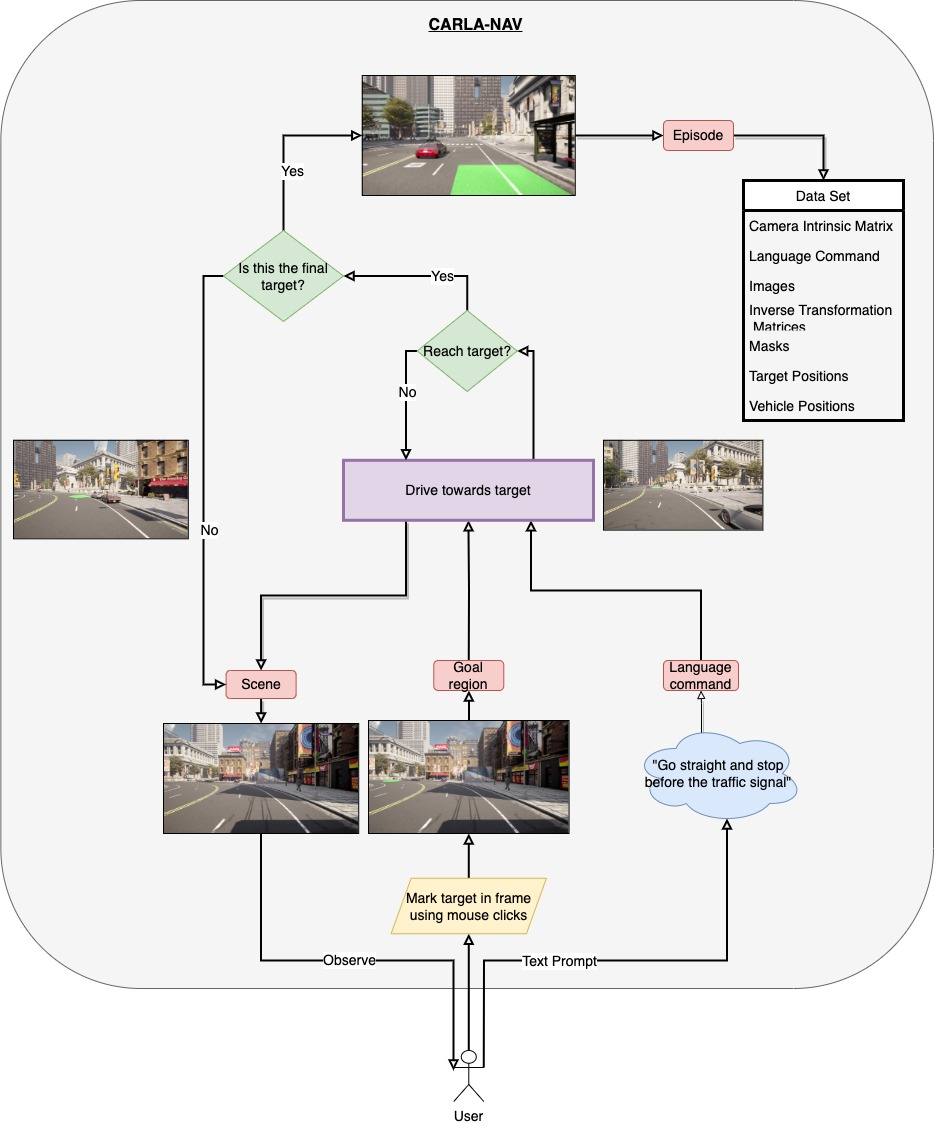
\includegraphics[width=0.48\textwidth]{images/data_set_updated_2.jpg}
\caption{TODO: Add suitable caption to data set pipeline.}
\label{pipeline}
\end{figure}

\section{Problem Statement}

Given a historical context of video frames $V=\{v_{t-k}, v_{t-k+1}, ... v_{t}\}$ and a language command $L = \{l_1, l_2, ...l_N\}$, where $t$ is the current timestamp, $k$ is the window size for historical frames and $N$ is the maximum number of words in the linguistic expression, the goal is to predict the navigable mask $y_t$ and the trajectory mask $z_t$ corresponding to the frame from current timestamp, ie: $v_t$. The spatial location of the navigation mask should determine the trajectory path's direction; similarly, the orientation of the trajectory path should determine the location of the navigable regions. In the next section we describe the network architecture and the training process.

% Given a sequence of video frames $V = \{v_1, v_2,..v_T\}$ and a language command $L = \{l_1, l2,..l_N\}$, the goal is to predict the navigable regions $\{y_1, y_2,..y_T\}$ and the trajectory masks $\{z_1, z_2,..z_T\}$ corresponding to each frame. The length of video is represented by $T$ and $N$ represents the maximum number of words in the command. The navigation masks $y_t$ and the trajectory mask $z_t$ for a given time step $t$ should be correlated with each other. The location of the navigation mask should determine the trajectory path's direction; similarly, the orientation of the trajectory path should determine the location of the navigable regions.


\section{Methodology}

We propose a novel multi-task network for navigation prediction and trajectory prediction tasks. Both tasks are treated as dense prediction tasks to make them interpretable for practical scenarios. We convert the dense pixel points to 3D world coordinates using inverse projective transformation during inference. The architecture for our model is illustrated in Figure~\ref{proposed_pipeline}. In the next section, we  describe the feature extraction process and the architecture in detail.

\textbf{Feature Extraction: }For the linguistic expression $L = \{l_1, l_2, ...l_N\}$, where $l_i$ is the $i^{th}$ word of the expression, we first compute the word embedding corresponding to each word using a pre-trained word embeddings. Following this, we pass the word embeddings through an LSTM to compute a word-level representation $F^l = \{f^{l}_{1}, f^{l}_{2}, ..., f^{l}_{N}\}$ of shape $\mathbb R^{B \times N \times C_l}$. For visual frames $V=\{v_{t-k}, v_{t-k+1}, ... v_{t}\}$, we utilize a 3D CNN backbone for extracting the video features $F^v=\{f^{v}_{t-k}, f^{v}_{t-k+1}, ... f^{v}_{t}\}$.

% \textbf{\emph{Frame-level Model: }} Our frame-level model 

% \textbf{\emph{Temporal Model: }} A sequence of video frames $V=\{v_{t-k}, v_{t-k+1}, ... v_{t}\}$ and the language command $L$  are passed as input to this network, and a 3D CNN backbone is used to extract video features. 

The input to our network are the video frames $V$ and the language command $L$. Specifically, for video $V$, we get visual features $F^v$ of shape $ \mathbb R^{C_v \times T \times HW}$, where H, W, T, and C represent the height, width, time, and channel dimensions, respectively. Following feature extraction, we apply joint multi-head self-attention over the spatial regions of frames and words of the command in the following manner,
\begin{equation} \label{eq1}
\begin{split}
    F &= F^v \odot F^l \\
    A &= \text{Mhead}(F, F, F)\\
    M &= A \ast F
\end{split}
\end{equation}

Here, $\odot$ represents the length-wise concatenation of the word-level linguistic features $F^l$ and the frame-level visual features $F^v$, $\text{Mhead}$ is the multi-head self-attention over the multi-modal features $F$ and $\ast$ represents the matrix multiplication. $M$ is the final multi-modal contextual feature with information from both visual and linguistic modalities.

Next, we describe the procedure for predicting the navigation and trajectory prediction masks. We want the future trajectory and the navigable region for the current time-step to be correlated with each other, ie: the future trajectory should point in the direction of the predicted navigable region. Consequently, we utilize the multi-modal contextual feature $M$ to predict the segmentation masks corresponding to the navigation and trajectory prediction tasks. For each task, we have a separate segmentation head, where each segmentation head comprises of sequence of convolution layers with upsampling operation. For training the segmentation masks, we utilize combo loss \cite{taghanaki2019combo} which is a combination of binary cross-entropy loss and dice loss:
\begin{equation} \label{eq2}
\begin{split}
    L_{bce} &= -{(y_{t}\log(\hat{y_{t}}) + (1 - y_{t})\log(1 - \hat{y_{t}}))}\\
    L_{dice} &= 2 * \frac{\hat{y_{t}} \cap y_{t}}{\Sigma{\hat{y_{t}}} + \Sigma{y_{t}}}\\        L_{combo} &= \lambda L_{bce} - (1 - \lambda) L_{dice}
\end{split}
\raisetag{3\normalbaselineskip}
\end{equation}

The proposed approach is end-end trainable and the predicted trajectory is highly correlated with the predicted navigation mask, as a result the predicted trajectory is interpretable in the sense that it captures the future route taken by the autonomous vehicle.

% dice loss + weighted cross entropy loss
% correlation by feature sharing -> nav mask, traj mask

% apply multi-head attention
% fusion -> dense prediction
% Two segmentation heads for mask prediction
% Navigation Mask Prediction
% Trajectory Mask Prediction

% Which loss function is used to train the multi-task network?

% Here, $\sigma$ is the softmax function, $\odot$ is matrix multiplication and $\ast$ is element-wise multiplication. $A \in \mathbb R^{T \times N}$ is cross-modal attention matrix between the image regions and the words of the command, $M \in \mathbb R^{T \times C}$ selects the relevant words corresponding to each spatial region in the image, and $f'_t \in \mathbb R^{T \times C}$ is the multi-modal feature corresponding to visual features $f_t$ and linguistic features $L$. Finally, $f'_t$ is passed through two separate decoders for predicting the segmentation masks corresponding to navigable regions and the future trajectory. Segmentation mask corresponding to the navigable regions contains two separate classes, one for intermediate navigable regions and the other for the final goal region. This is done to distinguish between the intermediate regions and final goal regions to identify the stopping criterion. Our full approach is end-end trainable.

\section{Experiments}

\textbf{Implementation Details: }We use X3D Architecture \cite{feichtenhofer2020x3d}, pre-trained on action recognition task on \cite{kay2017kinetics} for video feature extraction. The video frames are selected with a stride of $10$ and are resized to $224 \times 224$ resolution. After feature extraction, we get visual features of spatial resolution $H=W=7$ and channel dimension $C_v=512$. For linguistic features, we use GLoVe embeddings pre-trained on 840B tokens to initialize the word vectors, which are passed through LSTM to compute the word-level features corresponding to the linguistic command. Maximum length of command is set to $N=20$ and the channel dimension is $C_l=512$. We use batch size of 32 and our network is trained using AdamW optimizer, the initial learning rate is set to $1e^{-4}$ and polynomial learning rate decay with power of 0.5 is used.

\textbf{Evaluation Metrics:} We perform real-time evaluation in the Carla environment. Starting conditions are kept similar to that during validation data collection. The evaluation metrics used should compare the trajectory path during real-time evaluation with the ground truth trajectory during data collection. Thereby, we use \textbf{Frechet Distance} and normalized Dynamic Time Warping (\textbf{nDTW}) metrics to compare the predicted and the ground truth trajectories for the entire navigation task. \textbf{Eucledian Distance} metric is used to compare the trajectory endpoints. Additionally, \textbf{Task Completion} metric is used indicate the success rate of the language-based navigation task. For segmentation masks corresponding to final navigable regions and intermediate future trajectory, we use \textbf{Pointing Game} and \textbf{Recall@k} metrics described in \cite{Rufus_2021}. 

% \textbf{Proposed Model:} In the proposed model, we use a multi-frame segmentation and trajectory mask prediction model. We use X3D \cite{feichtenhofer2020x3d} pre-trained on Kinetics 400 dataset as backbone for visual feature extraction. The video input of with frames $T=40$ is used with stride $s=10$. The video frames are resized to $224 \times 224$ resolution and spatial resolution of extracted visual features is $H=7, W=7$. We pass the features output from the backbone to a 3D Convolutional Model that has a 

% \textbf{Baseline Model:} For Baseline, we use a per frame segmentation and trajectory mask prediction model. We use Vision Transformer \cite{dosovitskiy2020vit} pre-trained on Imagenet as backbone for visual feature extraction. Patch-size of $16 \times 16$ is used with hidden dimension $C=384$. The video frames are resized to $224 \times 224$ resolution and the spatial resolution of extracted visual features is $H=14, W=14$.

% We use 300 dimensional GLoVe embeddings to initialize the word vectors, which are passed through LSTM to compute the word-level features corresponding to the linguistic command. Maximum length of command is set to $T=20$. We use batch size of 32 and our network is trained using AdamW optimizer, the initial learning rate is set to $1e^{-4}$ and polynomial learning rate decay with power of 0.5 is used.


% \textbf{Evaluation Metrics:} We perform real-time evaluation in the Carla environment. Starting conditions are kept similar to that during validation data collection. The evaluation metrics used should compare the trajectory path during real-time evaluation with the ground truth trajectory during data collection. Thereby, we use \emph{Frechet Distance} metric to compare the trajectory curves and \emph{Eucledian Distance} metric is used to compare the trajectory endpoints. For segmentation masks corresponding to final navigable regions and future trajectory path, we use \emph{Pointing Game} and \emph{Recall@k} metrics described in \cite{Rufus_2021}. 

% Table
% Model  | Frechet Distance | nDTW | Eucledian | Task Completion | Pointing Game | Recall@K
% 
\subsection{Experimental Results}

We present the experimental results on all the evaluation metrics in this section.
% \subsubsection{Quantitative Results}


% Please add the following required packages to your document preamble:
% \usepackage{booktabs}
% \usepackage{multirow}
\begin{table}[]
    \begin{tabular}{@{}llll@{}}
    \toprule
    Metric                                          & Measure & Conv3D & VIT    \\ \midrule
    \multicolumn{1}{l|}{\multirow{3}{*}{Frechet}}   & Mean    & 17.836 & 43.945 \\
    \multicolumn{1}{l|}{}                           & STD     & 21.491 & 60.559 \\
    \multicolumn{1}{l|}{}                           & Median  & 9.101  & 12.187 \\ \cline{1-1}
    \multicolumn{1}{l|}{\multirow{3}{*}{FDE}}       & Mean    & 17.83  & 39.876 \\
    \multicolumn{1}{l|}{}                           & STD     & 21.496 & 51.379 \\
    \multicolumn{1}{l|}{}                           & Median  & 9.101  & 12.187 \\ \cline{1-1}
    \multicolumn{1}{l|}{\multirow{3}{*}{ADE}}       & Mean    & 10.307 & 22.097 \\
    \multicolumn{1}{l|}{}                           & STD     & 11.312 & 33.108 \\
    \multicolumn{1}{l|}{}                           & Median  & 5.77   & 7.106  \\ \cline{1-1}
    \multicolumn{1}{l|}{\multirow{3}{*}{ADE Match}} & Mean    & 4.728  & 16.433 \\
    \multicolumn{1}{l|}{}                           & STD     & 8.511  & 31.232 \\
    \multicolumn{1}{l|}{}                           & Median  & 1.259  & 2.5    \\ \bottomrule
    \end{tabular}
    \caption{Quantitative Results}
    \label{fig:quantitative}
\end{table}

% \textbf{Discrete Fr\'echet distance\cite{eifer1994frechet}} or \textbf{Coupling distance} is a discrete approximation of the Fr\'echet Distance. Fr\'echet distance gives the measure of similarity between curves taking into account the ordering of the curve.

% It is intuitively explained in \cite{eifer1994frechet} as ``A man is walking a dog on a leash: the man can move on one curve, the dog on the other; both may vary their speed, but backtracking is not allowed. What is the length of the shorted leash that is sufficient for traversing both curves?"

% \textbf{Definition} \textit{Fr\'echet distance}:
% Let $S$ be a metric space. A curve $A$ in $S$ is a continuous map from the unit interval into $S$, i.e., $A:[0,1] \to S$. A reparameterization of $\alpha$ [0,1] is continuous, non-decreasing, surjection $\alpha:[0,1]\to[0,1]$. Left $A$ and $B$ be two given curves in $S$. Then, the \textbf{Fr\'echet distance} between $A$ and $B$ is defined as the infimum over all reparameterizations $\alpha$ and $\beta$ of $[0,1]$ of the maximum over all $t\in[0,1]$ of the distance in $S$ between $A(\alpha(t))$ and $B(\beta(t))$. Thus, the Fr\'echet distance $F(A,B)$ is
% $$
% F(A,B) = \inf_{\alpha,\beta} \max_{t\in [0,1]} \left\{ d\left( A(\alpha(t)),B(\beta(t))\right)\right\}
% $$

% \textbf{Definition} \textit{Final Displacement Error(FDE)}
% Final Displacement error is defined as the $L2$ distance between the final trajectory points of the experimental and ground-truth trajectories.

% $$
% \textrm{FDE} = \sqrt{(x_T-x_T^{GT})^2+(y_T-y_T^{GT})^2}
% $$

% \textbf{Definition} \textit{Average Displacement Error(ADE)}
% Average Displacement error is defined as the mean $L2$ distance between all trajectory points of the experimental and ground-truth trajectories.

% $$
% \textrm{ADE} = \frac{1}{T} \sum_{i=1}^T\sqrt{(x_i-x_i^{GT})^2+(y_i-y_i^{GT})^2}
% $$

% Since ADE requires the trajectories compared to be of equal size, we define a metric \textbf{ADE-Match distance} to employ the dog-walking problem used in \textbf{Fr\'echet distance}. Thus we define \textbf{ADE-Match distance} as:

% \textbf{Definition} \textit{ADE-Match distance}:
% Let $S$ be a metric space. A curve $A$ in $S$ is a continuous map from the unit interval into $S$, i.e., $A:[0,1] \to S$. A reparameterization of $\alpha$ [0,1] is continuous, non-decreasing, surjection $\alpha:[0,1]\to[0,1]$. Left $A$ and $B$ be two given curves in $S$. Then, the \textbf{ADE-Match distance} between $A$ and $B$ is defined as the infimum over all reparameterizations $\alpha$ and $\beta$ of $[0,1]$ of the mean over all $t\in[0,1]$ of the distance in $S$ between $A(\alpha(t))$ and $B(\beta(t))$. Thus ADE-Match distance $AM(A,B)$ is
% $$
% AM(A,B) = \inf_{\alpha,\beta} \underset{t\in [0,1]}{\textrm{mean}} \left\{ d\left( A(\alpha(t)),B(\beta(t))\right)\right\}
% $$
% where $d(\textbf{p},\textbf{q})$ is the $L2$ distance between points $\textbf{p}$ and $\textbf{q}$.

\subsubsection{Qualitative Results}
Figure \ref{fig:qualitative_1} show the qualitative results for our trajectory masks.

\begin{figure}[h]
    \centering
    \begin{tabular}[t]{p{0.48\textwidth} }
    { \centering \small {\textit{\textbf{Command: }``Take a left from the intersection.''}}}\\
        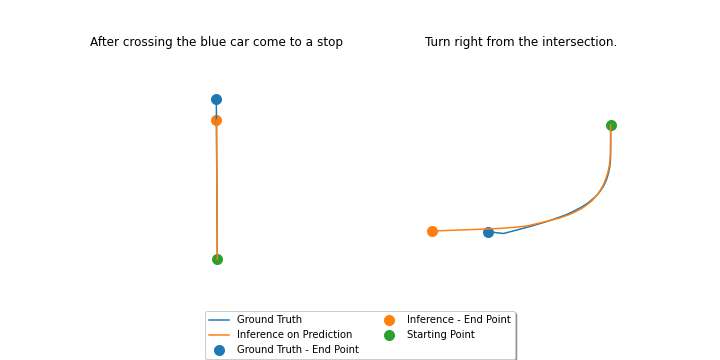
\includegraphics[width=0.48\textwidth]{images/qualitative_results.png} \\
        % \includegraphics[width=0.48\textwidth]{images/teaser2.jpg}\\
        % \includegraphics[width=0.48\textwidth]{images/teaser3.jpg}
    \end{tabular}
    \caption{Qualitative-1}
    \label{fig:qualitative_1}
\end{figure}

\begin{table*}[]
\centering
\begin{tabular}{@{}llllllll@{}}
\toprule
                                                      &           & \multicolumn{3}{l}{Conv3D} & \multicolumn{3}{l}{VIT}  \\ \midrule
Measure                                               &           & Mean    & Median  & STD    & Mean   & Median & STD    \\
\multicolumn{1}{l|}{Command Type}                    & Metric    &         &         &        &        &        &        \\ \cline{1-1}
\multicolumn{1}{l|}{\multirow{4}{*}{Stopping Based}} & Frechet   & 17.326  & 9.665   & 21.375 & 53.981 & 12.282 & 72.795 \\
\multicolumn{1}{l|}{}                                & FDE       & 17.316  & 9.665   & 21.383 & 47.667 & 12.282 & 60.744 \\
\multicolumn{1}{l|}{}                                & ADE       & 10.724  & 7.157   & 12.428 & 26.614 & 7.676  & 39.105 \\
\multicolumn{1}{l|}{}                                & ADE Match & 4.444   & 1.366   & 9.003  & 20.895 & 3.702  & 37.588 \\ \cline{1-1}
\multicolumn{1}{l|}{\multirow{4}{*}{Turning Based}}  & Frechet   & 17.97   & 6.965   & 21.371 & 36.416 & 16.678 & 40.996 \\
\multicolumn{1}{l|}{}                                & FDE       & 17.97   & 6.965   & 21.371 & 35.569 & 16.678 & 39.775 \\
\multicolumn{1}{l|}{}                                & ADE       & 10.017  & 5.041   & 9.3    & 17.524 & 10.15  & 21.721 \\
\multicolumn{1}{l|}{}                                & ADE Match & 5.033   & 1.321   & 7.565  & 11.398 & 3.451  & 18.248 \\ \bottomrule
\end{tabular}

    \caption{Based on Command Types}
    \label{fig:ablations_1}
\end{table*}
\begin{table*}
{
    \centering
    \begin{tabular*}{\textwidth}{@{}llllllll@{}}
    \toprule
    \multicolumn{2}{l}{}                                                 & \multicolumn{3}{l}{Conv3D} & \multicolumn{3}{l}{VIT}  \\ \midrule
    \multicolumn{2}{l}{Measure}                                          & Mean    & Median  & STD    & Mean   & Median & STD    \\
    \multicolumn{1}{l|}{Target Type}                         & Metric    &         &         &        &        &        &        \\ \cline{1-1}
    \multicolumn{1}{l|}{\multirow{4}{*}{infrastructure}}     & ADE       & 11.621  & 7.285   & 14.301 & 32.784 & 6.536  & 46.145 \\ 
    \multicolumn{1}{l|}{}                                    & ADE Match & 4.837   & 1.129   & 10.656 & 26.847 & 3.017  & 44.472 \\
    \multicolumn{1}{l|}{}                                    & FDE       & 16.792  & 9.44    & 19.272 & 55.207 & 12.044 & 70.361 \\
    \multicolumn{1}{l|}{}                                    & Frechet   & 16.807  & 9.44    & 19.259 & 64.845 & 12.044 & 85.244 \\ \cline{1-1}
    \multicolumn{1}{l|}{\multirow{4}{*}{road/traffic light}} & ADE       & 8.858   & 4.601   & 9.154  & 20.134 & 6.359  & 32.036 \\
    \multicolumn{1}{l|}{}                                    & ADE Match & 4.211   & 1.071   & 6.938  & 14.289 & 1.716  & 29.586 \\
    \multicolumn{1}{l|}{}                                    & FDE       & 15.635  & 7.521   & 19.475 & 33.312 & 12.694 & 37.973 \\
    \multicolumn{1}{l|}{}                                    & Frechet   & 15.635  & 7.521   & 19.475 & 38.849 & 12.694 & 53.439 \\ \cline{1-1}
    \multicolumn{1}{l|}{\multirow{4}{*}{automobile}}         & ADE       & 10.575  & 8.32    & 4.971  & 19.241 & 8.505  & 21.296 \\
    \multicolumn{1}{l|}{}                                    & ADE Match & 4.154   & 2.162   & 5.291  & 14.061 & 4.605  & 20.666 \\
    \multicolumn{1}{l|}{}                                    & FDE       & 25.478  & 13.31   & 34.689 & 47.479 & 22.171 & 45.582 \\
    \multicolumn{1}{l|}{}                                    & Frechet   & 25.478  & 13.31   & 34.689 & 47.479 & 22.171 & 45.582 \\ \bottomrule 
    \end{tabular*}
}
    \caption{Based on Object Reference in Command}
    \label{fig:ablations_3}
\end{table*}
% Please add the following required packages to your document preamble:
% \usepackage{booktabs}
% \usepackage{multirow}
\begin{table*}
\centering
\begin{tabular}{@{}llllllll@{}}
\toprule
                                         &           & \multicolumn{3}{l}{Conv3D} & \multicolumn{3}{l}{VIT}  \\ \midrule
Measure                                  &           & Mean    & Median  & STD    & Mean   & Median & STD    \\ 
\multicolumn{1}{l|}{Subcommand Counts}  & Metric    &         &         &        &        &        &        \\ \cline{1-1}
\multicolumn{1}{l|}{\multirow{4}{*}{1}} & ADE       & 12.133  & 7.221   & 12.934 & 23.256 & 7.995  & 30.824 \\
\multicolumn{1}{l|}{}                   & ADE Match & 6.052   & 1.285   & 9.954  & 17.297 & 3.817  & 28.929 \\
\multicolumn{1}{l|}{}                   & FDE       & 21.687  & 10.576  & 24.581 & 44.782 & 13.151 & 55.701 \\
\multicolumn{1}{l|}{}                   & Frechet   & 21.695  & 10.576  & 24.573 & 46.315 & 13.151 & 58.768 \\ \cline{1-1}
\multicolumn{1}{l|}{\multirow{4}{*}{2}} & ADE       & 6.427   & 4.655   & 5.132  & 19.636 & 4.743  & 38.485 \\
\multicolumn{1}{l|}{}                   & ADE Match & 1.914   & 1.193   & 2.494  & 14.598 & 1.26   & 36.605 \\
\multicolumn{1}{l|}{}                   & FDE       & 9.635   & 7.496   & 8.652  & 29.45  & 9.111  & 40.339 \\
\multicolumn{1}{l|}{}                   & Frechet   & 9.635   & 7.496   & 8.652  & 38.908 & 9.111  & 65.895 \\ \bottomrule
\end{tabular}
    \caption{Based on Number of Sub-command/Actions in the Command}
    \label{fig:ablations_4}
\end{table*}

\section{Real-time Navigation}


The toolkit allows using the learnt model in real time, using a synchronous CARLA environment which allows capture of frames from the RGB camera and process the outputs of network to predict the next target to be shared to the simple navigation planner. A rule based approach allows us to define the intermediate target locations which is derived from the predicted segmentation masks and the predicted trajectory. Another rule based method is employed to decide if the current predicted target location is the final position for a particular command or not.

The rule for determining the target location is as follows:
\begin{itemize}
    \item Set the counter for \textit{confident predictions} to 0
    \item Set the net segmentation map as mean of intermediate and final prediction masks.
    \item Threshold the net segmentation map.
    \item Divide the segmentation map into disconnected components.
    \item For the component with largest sum of probabilities, find the weighted centroid.
    \item If the sum of the values of the largest component in the target prediction mask is lower than a threshold $\delta_{\min}$, ignore the current prediction.
    \item If sum of the values of the largest component in the target prediction mask is higher than $\delta_{\max}$, use the weighted centroid as the next target.
    \item If sum of the values of the largest component in the target prediction mask is between $\delta_{\min}$ and $\delta_{\max}$, increment counter for \textit{confident predictions} by 1 and use the weighted centroid as the next target.
    
    \item Keep polling for next target prediction mask from the network until counter value for \textit{confident predictions} is less than 3.
    \item If the target is reached and there are no new targets for 3 seconds, end the run.

\end{itemize}

\bibliography{anthology,custom}
\bibliographystyle{acl_natbib}

\appendix

\section{Example Appendix}
\label{sec:appendix}

This is an appendix.

\end{document}
